\section{Experiments}
We evaluate our $\mathcal{T}C$-flow and $\mathcal{W}\mathbb{H}C$-flow in three settings. All of our model details, including hyperparameters and architectures can be found in Appendix \ref{model_arch_and_hyperparams}.

\xhdr{Setup and Baselines}
Throughout our experiments we rely on three main baselines which we use to compare against normalizing flows constructed using $\mathcal{T}C$ and $\mathcal{W}\mathbb{H}C$ layers. In Euclidean space we use Gaussian latent variables and affine coupling flows, denoted $\mathcal{N}$ and $\mathcal{N}C$ respectively. As we operate in the Lorentz model we further define Wrapped Gaussians latent variables, $\mathbb{H}$, in this space as an appropriate baseline. Due to the fact that all model parameters are defined on tangent spaces they are easily optimized using conventional Euclidean space optimizers like Adam \cite{kingma2014adam}, which we use for all models. Similar to prior work we also consider the curvature $K$ as a learnable parameter with a warmup of $10$ epochs that progressively increasing curvature \cite{skopek2019mixed}.


\subsection{Structured Density Estimation}
We first consider structured density estimation in a canonical VAE setting. In this setting, we seek to learn rich approximate posteriors using normalizing flows and we evaluate the negative test marginal log-likelihood of data. We evaluate our normalizing flow on a Branching Diffusion Process (BDP) \cite{mathieu2019continuous} which is binary tree with injected and Dynamically binarized MNIST \cite{skopek2019mixed}. Our results are shown in Tables \ref{bdp_embeddings_table} and \ref{mnist_embeddings_table} and we observe significant gains on both datasets when the latent dimension is small. In particular, $\mathcal{W}\mathbb{H}C$ performs the best with 2 dimensional latents with an relative improvement of \red{\%XX} over $\mathcal{N}C$ normalizing flows. We reconcile this result by recalling that even in two dimensions hyperbolic spaces have more room to embed hierarchies. As we increase the latent dimension however we see that Euclidean based approaches outperform our proposed models which is line with similar observation in prior work \cite{nickel2017poincare}.
\begin{table}[ht]
\label{bdp_embeddings_table}
\begin{small}
\begin{center}
\begin{tabular}{lccccr}
    \toprule
    Model   &  BDP-2 & BDP-4 & BDP-6\\
    \midrule
    $\mathcal{N}$-VAE & $-55.4_{\pm 0.2}$  & $-55.2_{\pm 0.3}$& $-56.1_{\pm 0.2}$   \\
    $\mathbb{H}$-VAE & $-54.9_{\pm 0.3}$& $-55.4_{\pm 0.2}$ &  $-58.0_{\pm 0.2}$\\
    \cut{$\mathcal{P}$-VAE$^*$ & $-55.6_{\pm 0.2}$ & - &-  \\}
    \cut{$\mathbb{U}$-VAE & &  & $-55.8_{\pm 0.4}$  \\}
    $\mathcal{N}C$ & $-55.4_{\pm 0.4}$ & $ \textbf{-54.7}_{\pm 0.1}$ & $\textbf{-55.2}_{\pm 0.3}$  \\
    $\mathcal{T}C$& $-54.9_{\pm 0.1}$& $-55.6_{\pm 0.2}$& $-57.5_{\pm0.2}$\\
    $\mathcal{W}\mathbb{H}C$& $\textbf{-52.8}_{\pm 0.3}$ & $-55.2_{\pm 0.2}$& $-57.4_{\pm 0.3}$\\
    \bottomrule
\end{tabular}
\caption{Test Log Likelihood on Binary Diffusion Process versus latent dimension. All normalizing flows use 2-coupling layers.}
\end{center}
\vskip -0.1in
\end{small}
\end{table}

\begin{table}[ht]
\label{mnist_embeddings_table}
\begin{small}
\begin{center}
\begin{tabular}{lcccc}
    \toprule
    Model   &  \shortstack{MNIST\\2} & \shortstack{MNIST\\4} & \shortstack{MNIST\\6}  \\
    \midrule
    $\mathcal{N}$-VAE &$-139.5_{\pm 1.0}$& $-115.6_{\pm0.2}$ & $-100.0_{\pm0.02}$ \\
    $\mathbb{H}$-VAE & $*$ & $-113.68_{\pm0.9}$& $-99.8_{\pm0.2}$ \\
    \cut{$\mathcal{P}$-VAE$^*$ & $-142.5_{\pm 0.4}$ & $-97.7_{\pm0.2}$&  \\}
    \cut{$\mathbb{U}$-VAE$^*$ & - & $-97.3_{\pm 0.2}$ &  \\}
    $\mathcal{N}C$ &  $-139.2_{\pm 0.4}$ & $-115.2_{\pm0.6}$& $\textbf{-98.7}_{0.3}$ \\
    $\mathcal{T}C$  & $*$& $ \textbf{-112.5}_{\pm0.2}$&$-99.3_{\pm0.2}$  \\
    $\mathcal{W}\mathbb{H}C$ & $\textbf{-136.5}_{\pm 2.1}$ & $-112.8_{\pm0.5}$ &$-99.4_{\pm0.2}$ \\
    \bottomrule
\end{tabular}
\caption{Test Log Likelihood on MNIST averaged over 5 runs verus latent dimension. * indicates numerically unstable settings.}
\end{center}
\vskip -0.1in
\vspace{-10pt}
\end{small}
\end{table}

\subsection{Graph Reconstruction}
We conduct experiments on the task of link prediction in graph with a GNN-based inference model. Specifically, given a simple graph $\mathcal{G}=(\V,A, X)$, defined by a set of nodes $\mathcal{V}$, an adjacency matrix $A \in \mathbb{Z}^{|\mathcal{V}| \times |\mathcal{V}|}$ and node feature matrix $X \in \mathbb{R}^{\mathcal{V} \times n}$, we learn a VGAE \cite{kipf2016variational} model whose inference network, $q_\phi$, defines a distribution over node embeddings $q_\phi(Z | A, X)$. To score the likelihood of an edge existing between pairs of nodes we use a inner product decoder, ---i.e.$p(A_{u,v}=1|z_u,z_v) = \sigma(z_u^Tz_v)$,  by first mapping the node embeddings to $\mathcal{T}_{\textbf{o}}\mathbb{H}^n_K$. Given these components, the inference GNNs are trained to minimize the variational lower bound on a training set of edges. 

We use two different Diesease datasets taken from \citep{chami2019hyperbolic} and \citep{mathieu2019continuous} for evaluation purposes. The first dataset Diseases-\RNum{1} is composed of a network of disorders and disease genes linked by known disorder–gene associations \cite{goh2007human}. In the second dataset Diseases-\RNum{2}, we build tree networks of an SIR disease spreading model \cite{anderson1992infectious}, where node features determine the susceptibility to the disease. In Table \ref{graph_embeddings_table} we report Test AUC and Test AP, where the improved performance of the model $\mathcal{W}\mathbb{H}C$ can be observed. Similar to the structured density estimation setting, the performance gains of $\mathcal{W}\mathbb{H}C$ are best observed in low-dimensional latent spaces.


% In the first dataset, Diseases-\RNum{1}, we build tree networks of an SIR disease spreading model \cite{anderson1992infectious}, where node features determine the susceptibility to the disease. In Diseases-\RNum{2}, contains a network of disorders and disease genes linked by known disorder–gene associations \cite{goh2007human}. 

% \joey{Ariella can you just briefly comment on the empirical numbers here. Diesease-1 and 2 are LP and the other respectively.}

% \begin{table}[ht]
% \label{graph_embeddings_table}
% \begin{small}
% \begin{center}
% \begin{tabular}{lcccc}
%     \toprule
%     Model   & \shortstack{Dis-\RNum{1}\\AUC} & \shortstack{Dis-\RNum{1}\\AP}  & \shortstack{Dis-\RNum{2}\\AUC} & \shortstack{Dis-\RNum{1}\\AP}  \\
%     \midrule
%     $\mathcal{N}$-VAE & $0.89_{\pm 0.02}$ &
%     $0.91_{\pm 0.01}$ &
%     $0.92_{\pm 0.01}$ &
%     $0.91_{\pm 0.01}$ 
    
%     \\
%     $\mathbb{H}$-VAE & $0.90_{\pm 0.01}$ &
%     $0.91_{\pm 0.01}$ &
%     $0.92_{\pm 0.00}$ &
%     $0.91_{\pm 0.01}$ 
    
%     \\
%     $\mathcal{N}C$ & $0.91_{\pm 0.01}$ &
%     $0.92_{\pm 0.01}$ &
%     $0.95_{\pm 0.00}$ &
%     $0.93_{\pm 0.01}$ 
    
%     \\
%     $\mathcal{T}C$ & $\textbf{0.93}_{\pm 0.01}$&
%     $\textbf{0.93}_{\pm 0.00}$ &
%     $\textbf{0.96}_{\pm 0.01}$ &
%     $0.95_{\pm 0.01}$ 
    
%     \\
%     $\mathcal{W}\mathbb{H}C$ & $0.93_{\pm 0.01}$&
%     $0.92_{\pm 0.01}$ &
%     $\textbf{0.96}_{\pm 0.01}$ &
%     $\textbf{0.96}_{\pm 0.01}$ 
%     \\
%     \bottomrule
% \end{tabular}
% \end{center}
% \end{small}
% \caption{Test AUC and Test AP on Graph Embeddings where Dis-\RNum{1} has latent dimesion 6 and Dis-\RNum{2} has latent dimension 2.}
% \vskip -0.1in
% \end{table}

\begin{table}[ht]
\label{graph_embeddings_table}
\begin{small}
\begin{center}
\begin{tabular}{lcccc}
    \toprule
    Model   & \shortstack{Dis-\RNum{1}\\AUC} & \shortstack{Dis-\RNum{1}\\AP}  & \shortstack{Dis-\RNum{2}\\AUC} & \shortstack{Dis-\RNum{2}\\AP}  \\
    \midrule
    $\mathcal{N}$-VAE & $0.90_{\pm 0.01}$ &
    $0.92_{\pm 0.01}$ &
    $0.92_{\pm 0.01}$ &
    $0.91_{\pm 0.01}$
    
    \\
    $\mathbb{H}$-VAE & $0.91_{\pm 5\textnormal{e-3}}$ &
    $0.92_{\pm 5\textnormal{e-3}}$ &
    $0.92_{\pm 4\textnormal{e-3}}$ &
    $0.91_{\pm 0.01}$ 
    
    \\
    $\mathcal{N}C$ & $0.92_{\pm 0.01}$ &
    $0.93_{\pm 0.01}$ &
     $0.95_{\pm 4\textnormal{e-3}}$ &
    $0.93_{\pm 0.01}$ 
    
    \\
    $\mathcal{T}C$ & $\textbf{0.93}_{\pm 0.01}$ &
    $0.93_{\pm 0.01}$ &
   $\textbf{0.96}_{\pm 0.01}$ &
     $0.95_{\pm 0.01}$ 
    
    \\
    $\mathcal{W}\mathbb{H}C$ & $\textbf{0.93}_{\pm 0.01}$&
    $\textbf{0.94}_{\pm 0.01}$ &
    $\textbf{0.96}_{\pm 0.01}$ &
    $\textbf{0.96}_{\pm 0.01}$
    \\
    \bottomrule
\end{tabular}
\end{center}
\end{small}
\caption{Test AUC and Test AP on Graph Embeddings where Dis-\RNum{1} has latent dimesion 6 and Dis-\RNum{2} has latent dimension 2.}
\vskip -0.1in
\end{table}

\subsection{Graph Generation}
We now turn to the graph generation setting where we construct two synthetic datasets containing lobster graphs and random trees generated using prufer sequences. We follow the two stage training procedure outlined in Graph Normalizing Flows \cite{liu2019graph} in that we first train a deterministic autoencoder. Empirically, we find that defining edge probabilities using a distance based decoder consistently leads to better generation performance. Thus we define edge probabilities as, $p(A_{u,v}=1|z_u,z_v) = \sigma((-d_{\mathcal{G}}(u,v) - b)/\tau)$ where $b$ and $\tau$ are learned edge specific bias and temperature parameters. Starting from these fixed node embeddings we then train normalizing flows for density estimation. To model dependencies between node embeddings we use GRevNets \cite{liu2019graph} and an analagous version in hyperbolic space with graph attention \cite{velivckovic2017graph}. At inference time, we we first sample the number of nodes to generate from the empirical distribution of the dataset. We then independently sample node latents from our prior distribution and begin with a fully connected graph and then run our normalizing flow to give refined edge probabilities. 

\begin{figure*}
    \centering
    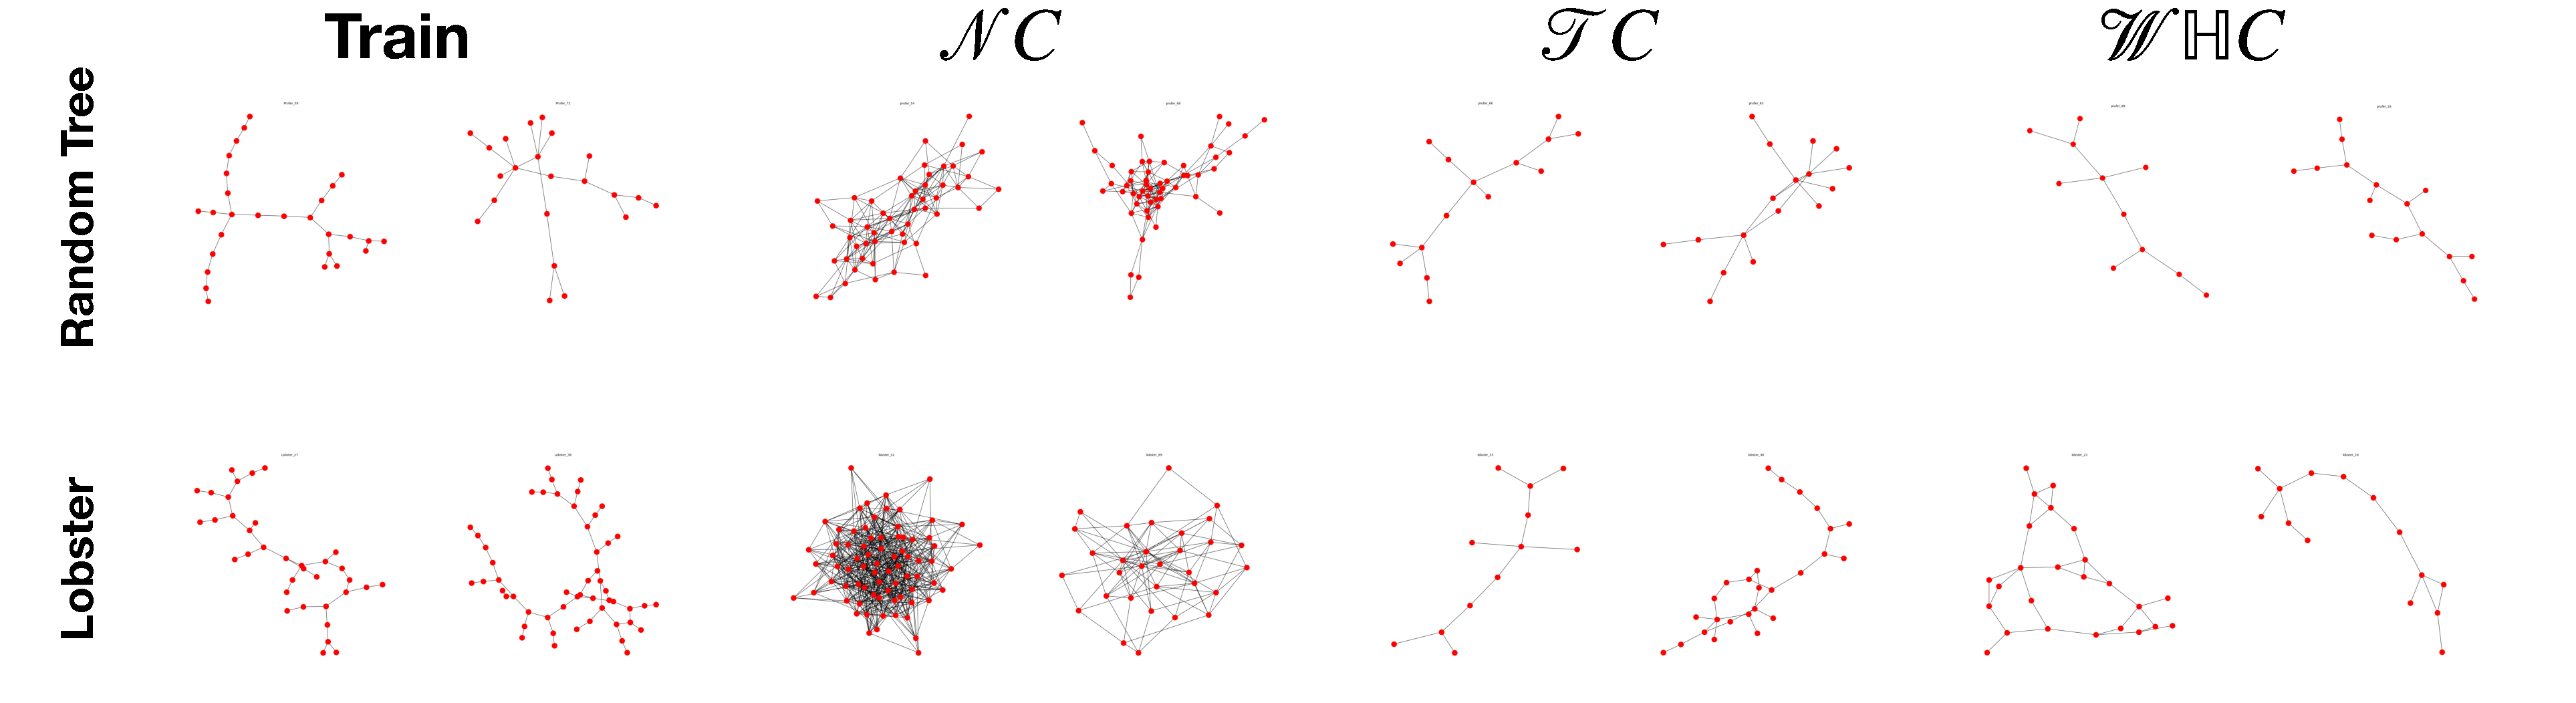
\includegraphics[width=\textwidth]{hyperbolic_graph_gen.pdf}
    \vspace{-5mm}
    \caption{Selected qualitative results on graph generation for lobster and random tree graph.}
    \label{fig:graph_generation_pic}
\end{figure*}

Our evaluation setup closely mirrors that of \cite{liao2019efficient} in that we construct $100$ training graphs with minimum and maximum number of nodes of $20$ and $100$ respectively, and calculate mean maximum discrepancy between distributions of graph statistics for generated and ground truth graphs. In table \ref{graph_gen_table} we present quantitative results for both datasets while Fig. \ref{fig:graph_generation_pic} shows selected generated samples.\cut{and find that both $\mathcal{T}C$ and $\mathcal{W}\mathbb{H}C$ achieve lower MMD scores on all metrics aside from clustering coefficient on Lobster graphs but achieves higher MMD scores on random trees.} As shown in Fig. \ref{fig:graph_generation_pic} generated samples using $\mathcal{N}C$ for the random trees dataset are simply shallow trees with only a handful of nodes which trivially have low MMD scores but do not respect the structure in the data. For lobster graphs, $\mathcal{N}C$ resembles closer to a fully connected graph and is unable to distinguish the hierarchy in the data. These empiricial observations are corroborated in the MMD metrics where we find that both $\mathcal{T}C$ and $\mathcal{W}\mathbb{H}C$ achieve lower MMD scorest. Critically, a significantly higher proportion of generated samples are actually lobster graphs, while none of the samples generated by $\mathcal{N}C$ respect this hierarchical structure. \cut{Critically, samples generated by the different normalizing flow models demonstrate that flows on hyperbolic spaces are better able to capture the hierarchical structure of data with deeper hierarchies. Critically, a significantly higher proportion of generated samples are actually lobster graphs, while none of the samples generated by $\mathcal{N}C$ respect this hierarchical structure. Fig. \ref{fig:graph_generation_pic} shows selected s}

\begin{table*}[]
\label{graph_gen_table}
\begin{scriptsize}
\begin{center}
\begin{tabular}{lllllllllll}
    \toprule
     & \multicolumn{5}{c}{Prufer} &  \multicolumn{5}{c}{Lobster} \\
    
    \midrule
    Model   & Deg. & Clus. & Orb. & Spec. & Acc. & Deg. & Clus. & Orb. & Spec. & Acc.\\
    \midrule
    $\mathcal{N}C$ &$\textbf{0.30}_{\pm0.12}$ & $\textbf{0.59}_{\pm0.40}$& $\textbf{0.57}_{\pm0.38}$& $\textbf{0.31}_{\pm0.15}$ & $\textbf{26.0}_{\pm25.0}$ & $0.47_{\pm3.0\textnormal{e-3}}$ & $1.02_{\pm7.6\textnormal{e-3}}$& $0.28_{\pm0.37}$& $0.50_{\pm0.01}$ & $0.00_{\pm0.0}$  \\
    $\mathcal{T}C$ & $0.31_{\pm0.09}$ & $1.01_{0.29}$& $0.89_{\pm0.11}$& $0.35_{\pm0.09}$ & $5.0_{\pm4.5}$ & $\textbf{0.39}_{\pm0.07}$ & $1.02_{0.62}$& $0.75_{\pm0.38}$& $0.40_{\pm0.11}$ & $\textbf{17.4}_{\pm33.7}$\\
    $\mathcal{W}\mathbb{H}C$ & $0.31_{\pm0.14}$ & $0.72_{\pm0.33}$&  $0.72_{\pm0.33}$& $0.32_{\pm0.14}$ & $16.3_{\pm20.9}$ & $0.41_{\pm0.07}$ & $\textbf{0.96}_{\pm0.43}$& $\textbf{0.47}_{\pm0.44}$& $\textbf{0.39}_{\pm0.13}$ & $11.8_{\pm23.1}$\\
    \bottomrule
\end{tabular}
\end{center}
\caption{Prufer and Lobster.}
\vskip -0.1in
\end{scriptsize}
\end{table*}
%cccccccccc
